\documentclass[10pt]{beamer}

\usepackage{enumerate}
\usepackage{graphicx}
\usepackage{amsmath}
\usepackage{ragged2e}
\usepackage[utf8]{inputenc}
\usepackage[ngerman]{babel}
\usepackage{sidecap}

\mode<beamer>{
\usetheme[subsectionstyle=hide, compress]{Dresden}
\usecolortheme{sidebartab}
\setbeamertemplate{itemize subitem}[circle]
%\beamertemplatenavigationsymbolsempty
}


\title[Abschlusspr\"asentation]{Abschlusspr\"asentation PPG5}
\subtitle{WS 2009 / 2010}
\author[PPG5]{Michele Collodo, Andreas Glossner, Karl-Christoph G\"odel,\\Bastian Hacker, Maria Obst, Alexander Wagner, David Winnekens}
\date{04. Februar 2010}

\begin{document}

\frame
{
\hfill

\includegraphics[width=0.20\textwidth]{images/ppg5logocrop.pdf}
\titlepage
}

%%%%%%%%%%%%%%%%%%%%%%%%%%%%%%%%%%%%%%%%%%%%%%%%%%%%%%%%%%%%%%%%%%%%%%%%%%%%%%%%%%%%%%%%%%%%%%%%%%%%%%%%%%%%%%%%
\section{LED-Spektrometer}
\subsection[]{Grundidee}
\frame
{
\frametitle{Grundidee}
\begin{figure}
\begin{center}
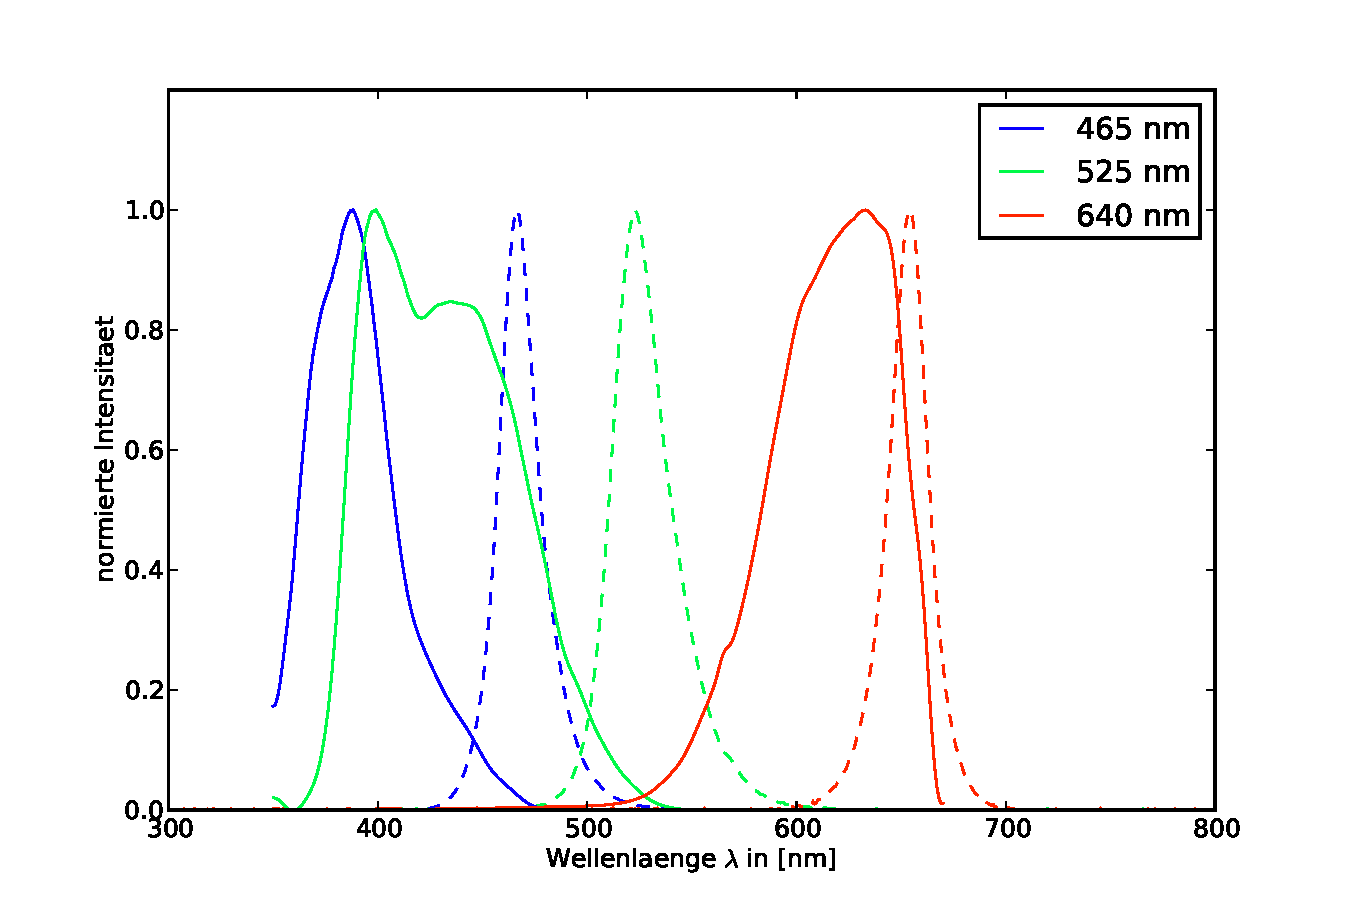
\includegraphics[width=0.8\textwidth]{./images/absorp-emit.pdf}
\caption{Verschiedenfarbige LEDs mit verschiedenen Absorptionsspektren}
\end{center}
\end{figure}
}

\subsection[]{Vorgehen}
\frame
{
\frametitle{Vorgehen}
\begin{enumerate}
\item Vormessungen
\item Elektronik
\item Software 
\end{enumerate}

\begin{figure}
\begin{center}
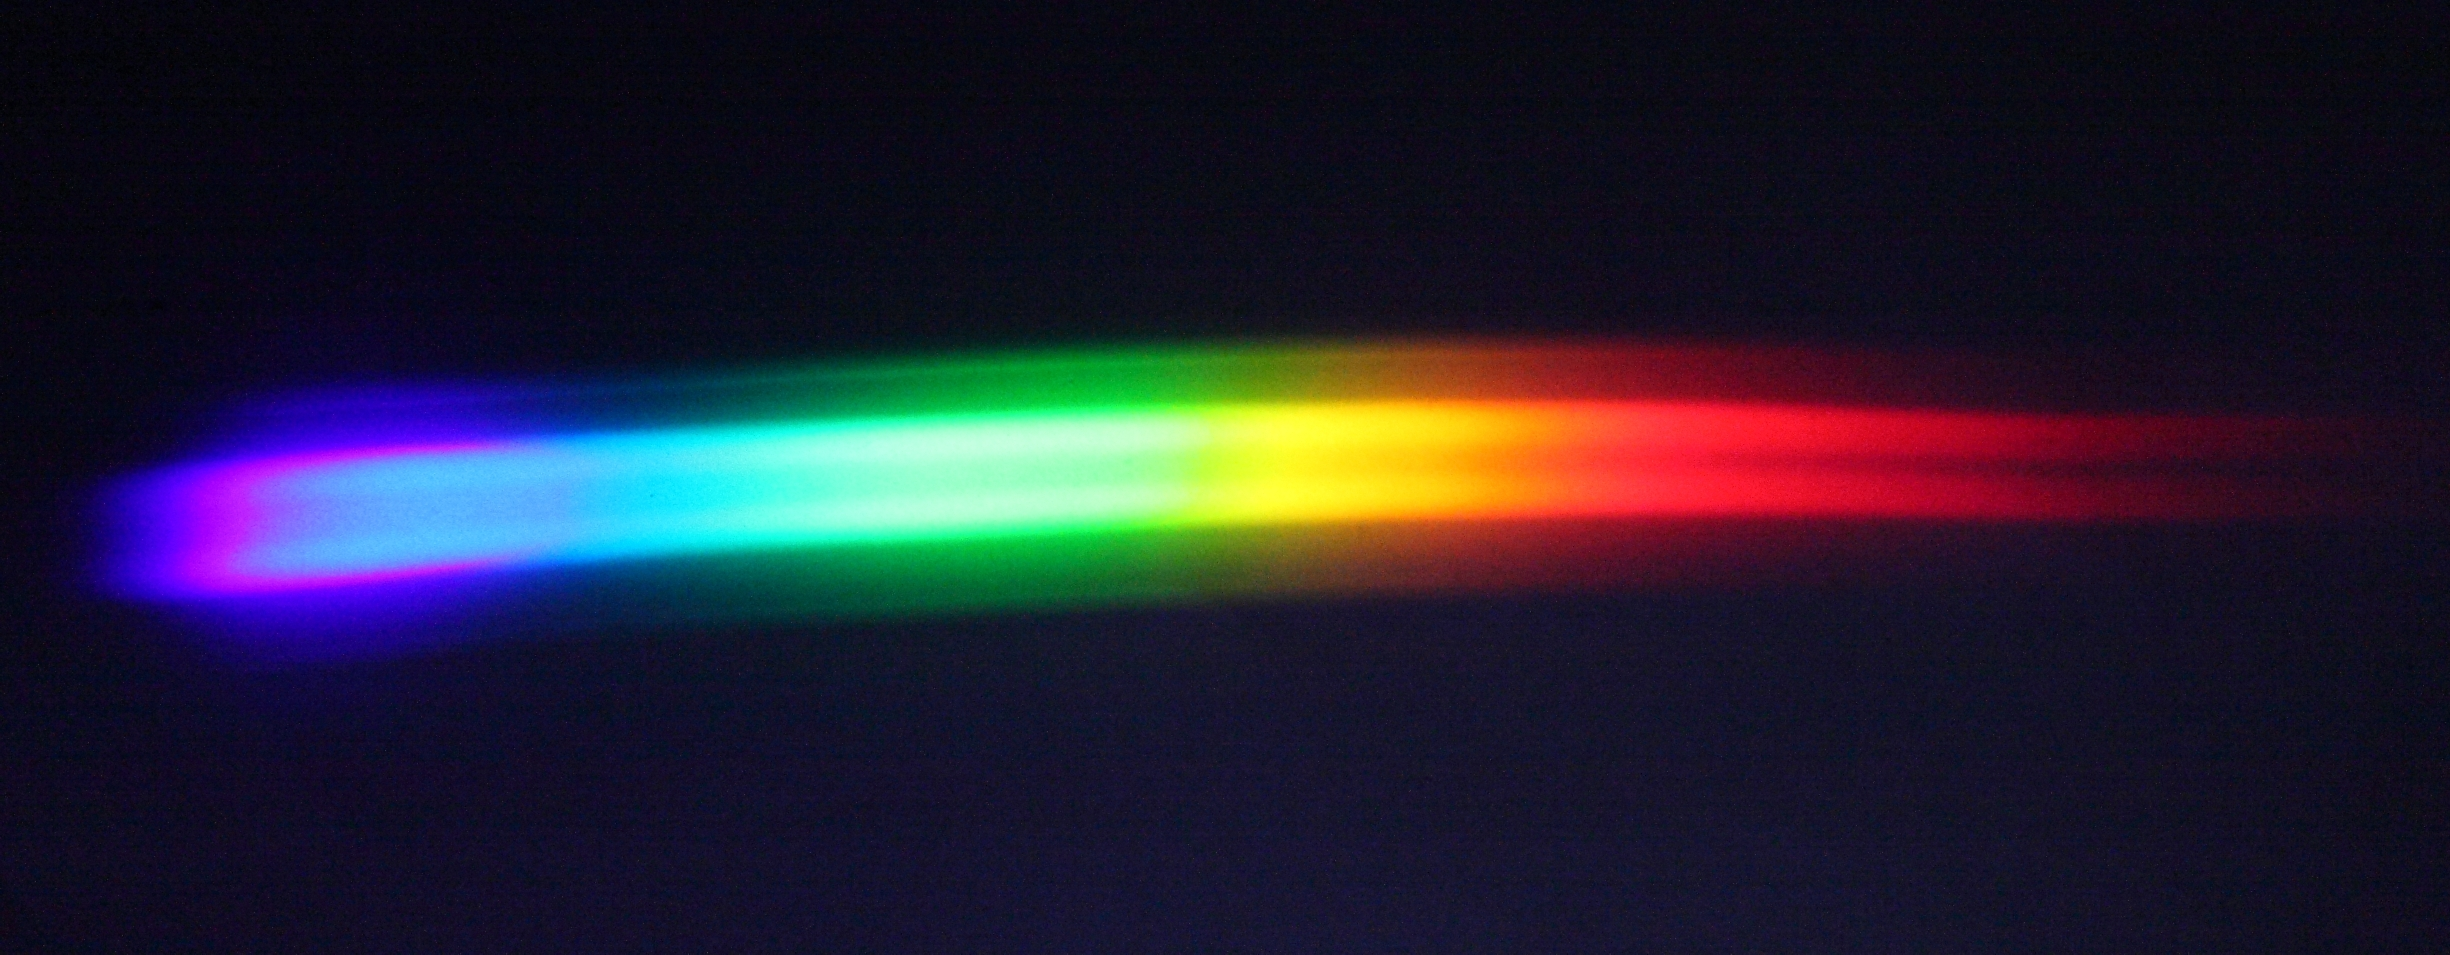
\includegraphics[width=\textwidth]{./images/spektrum_web.jpg}
\end{center}
\end{figure}
}
\frame
{
\frametitle{Vormessungen I}
\begin{figure}
\begin{center}
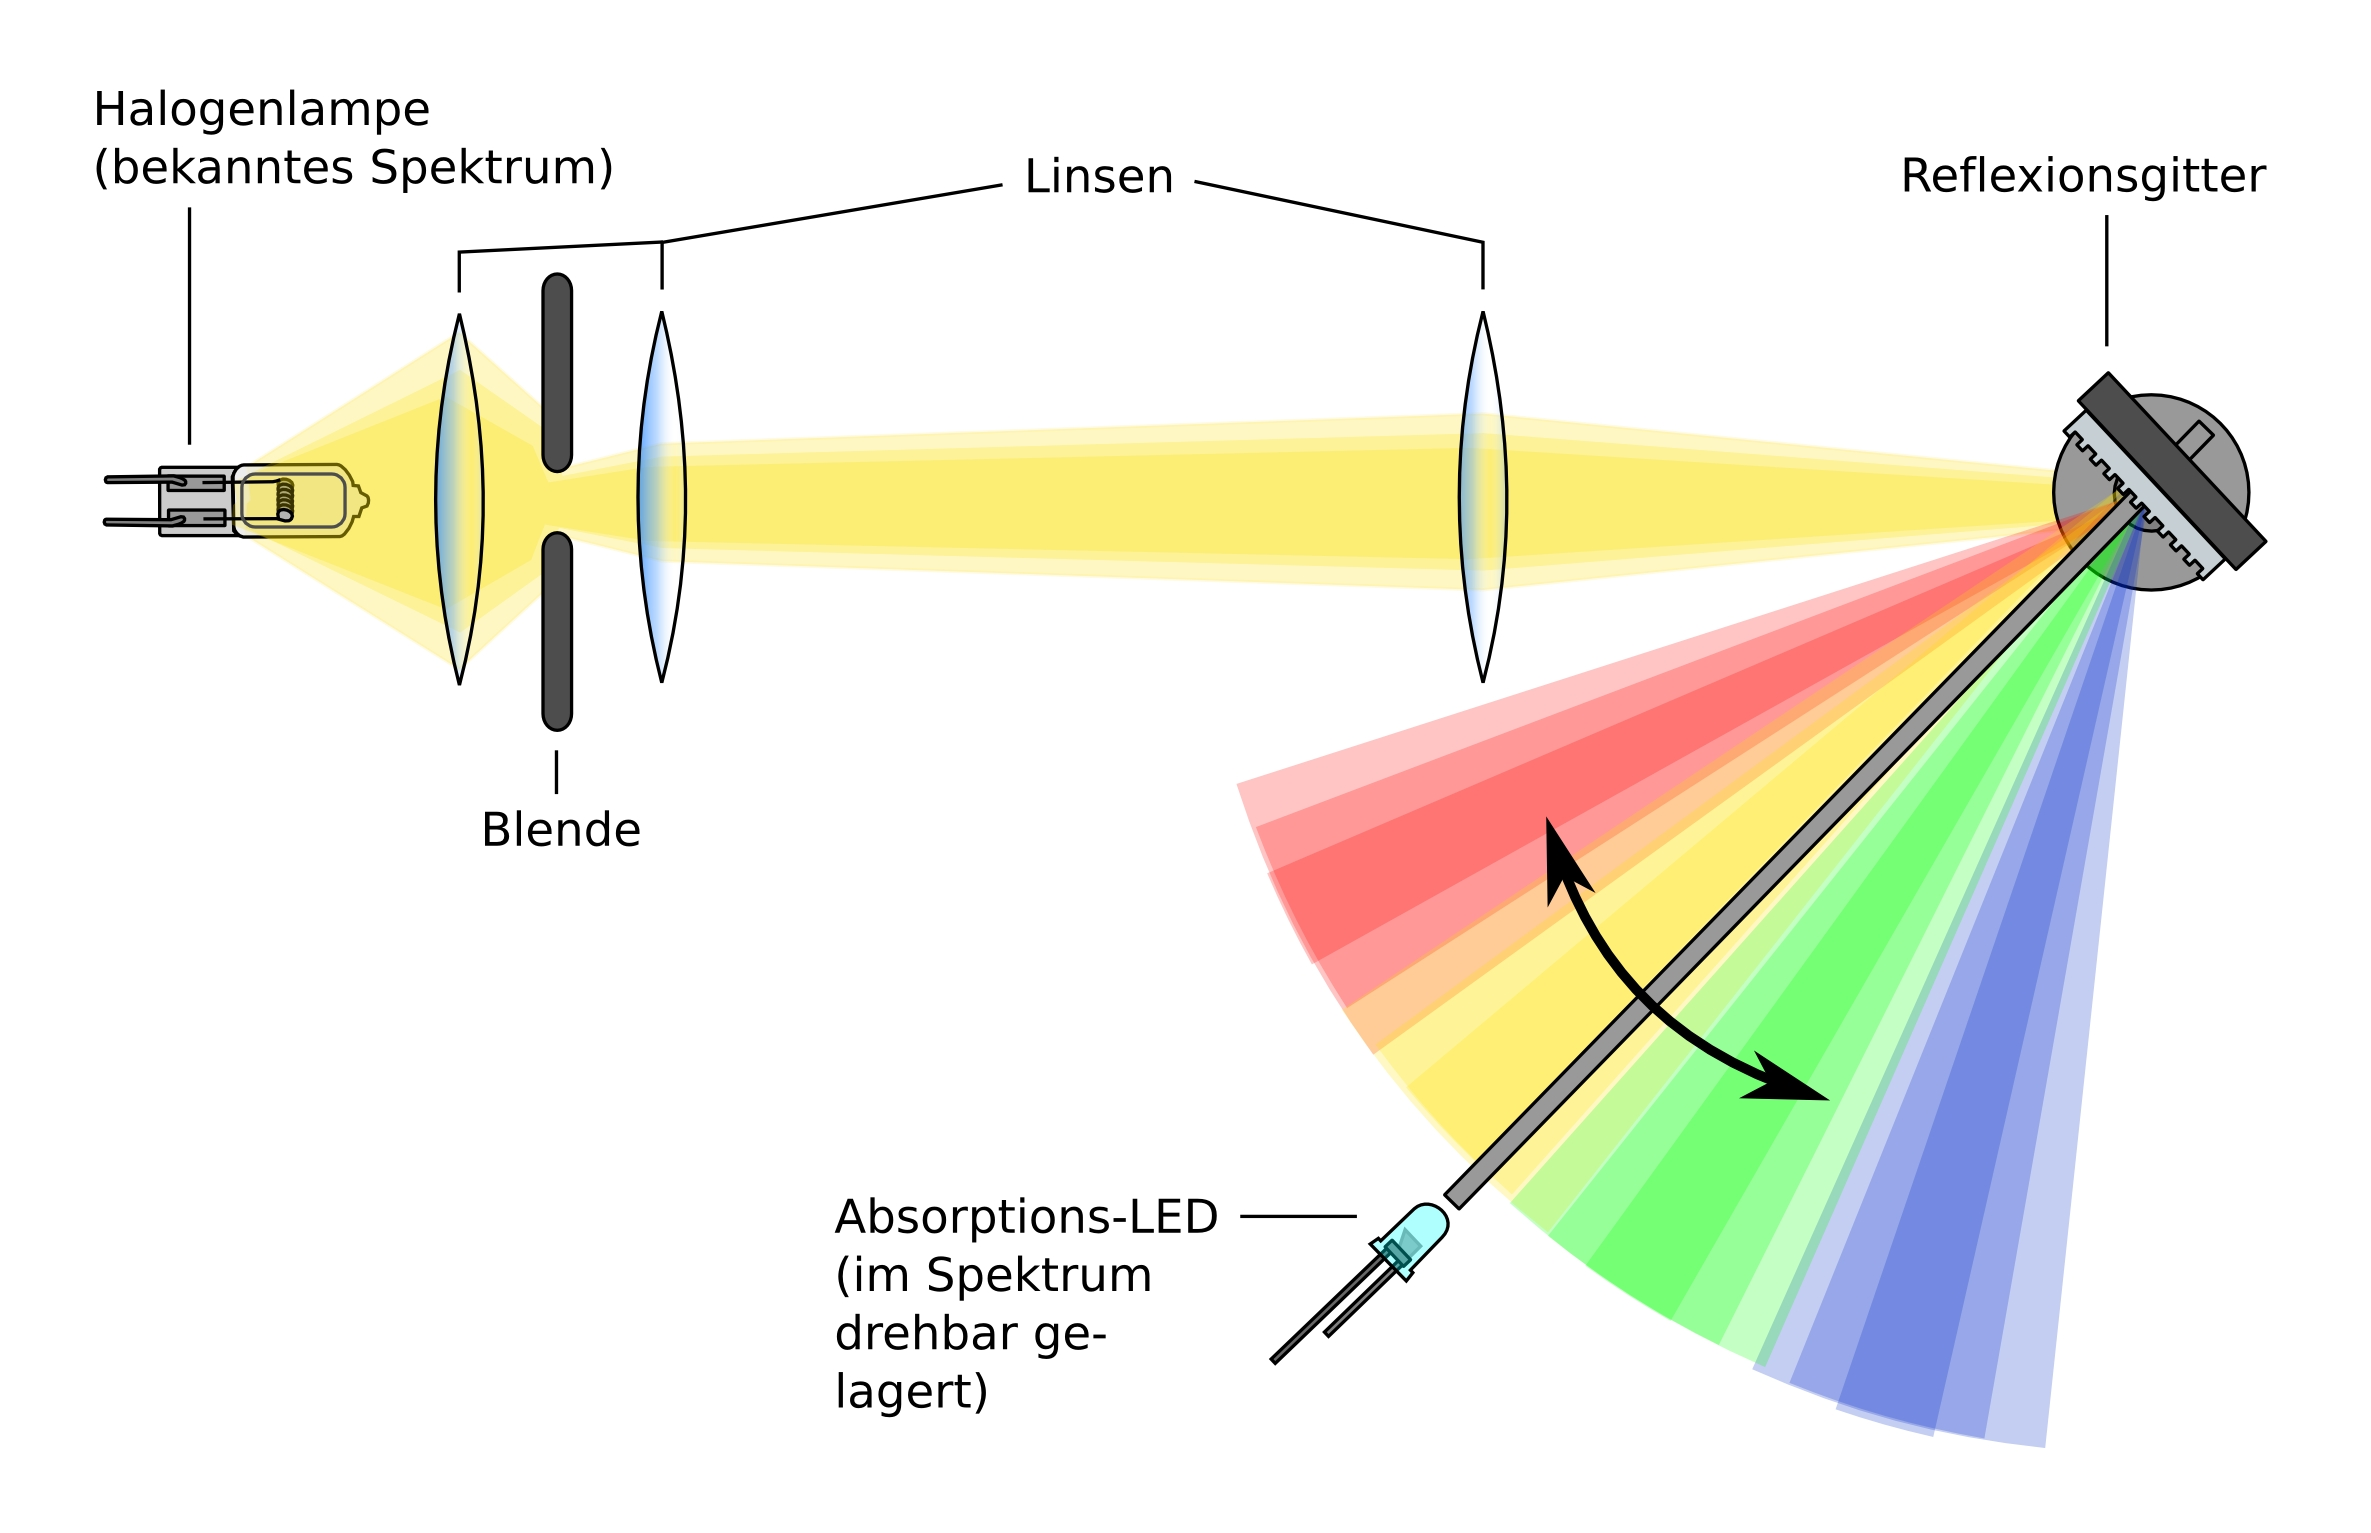
\includegraphics[width=0.8\textwidth]{./images/setup.jpg}
\caption{Aufbau f\"ur die Kalibration}
\end{center}
\end{figure}
}
\frame
{
\frametitle{Vormessungen II}
\begin{figure}
\begin{center}
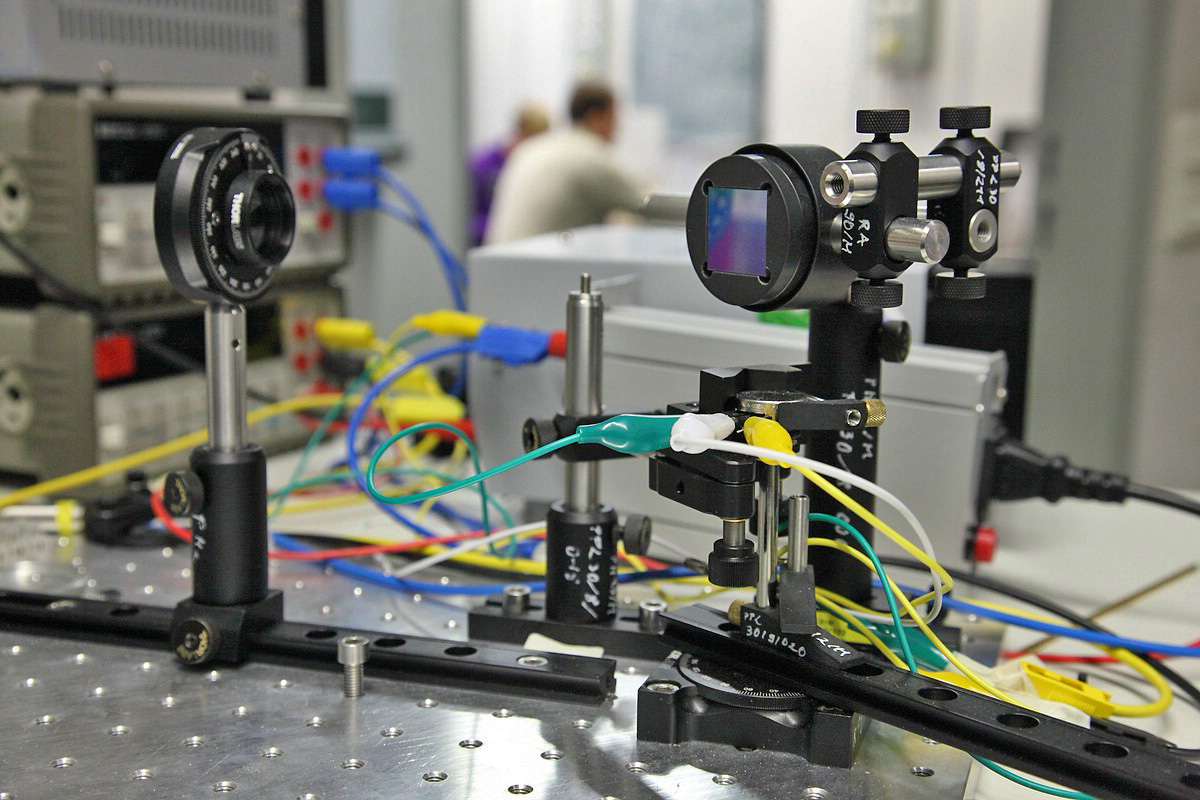
\includegraphics[width=0.8\textwidth]{./images/prIMG_7244bh}
\caption{Kontinuierliche Winkelmessung}
\end{center}
\end{figure}
}
\frame
{
\frametitle{Elektronik}
\begin{figure}
\begin{center}
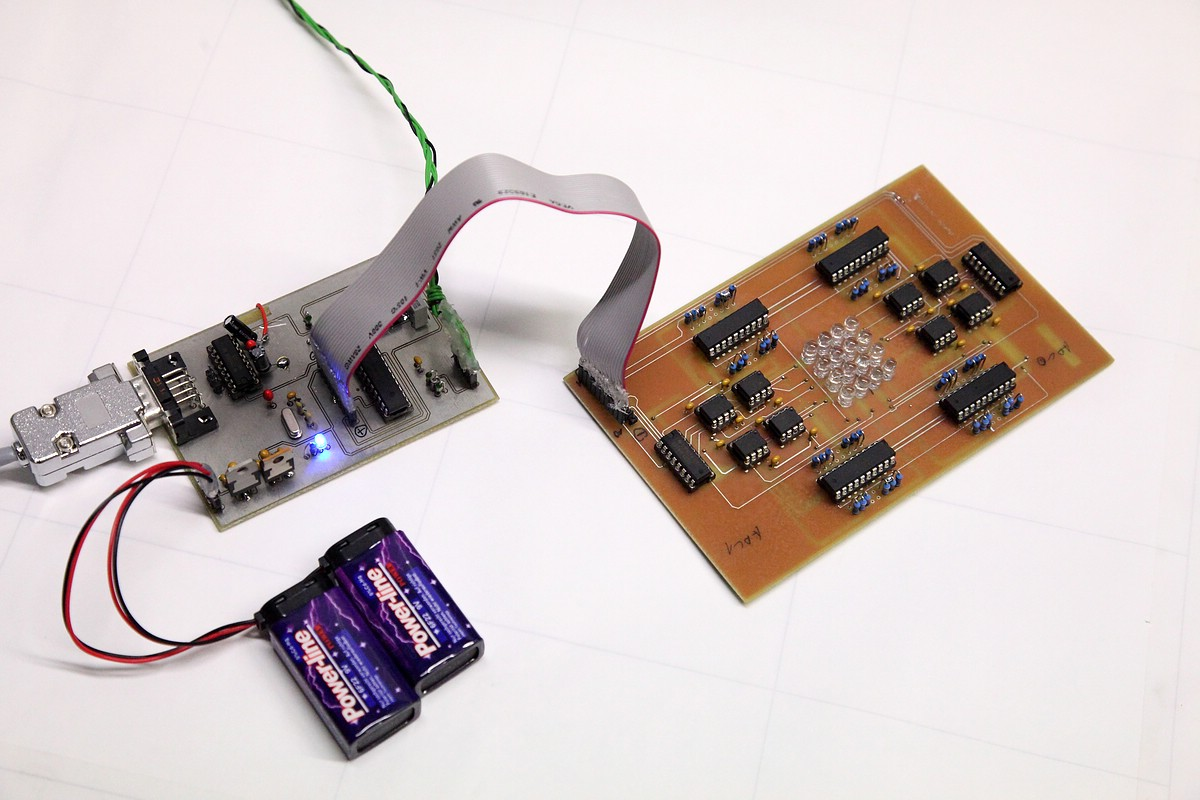
\includegraphics[width=0.8\textwidth]{./images/elektronik-final.jpg}
\caption{Das fertige LED-Spektrometer}
\end{center}
\end{figure}
}

\frame
{
\frametitle{Software}
\begin{block}{Python Programm zur Auswertung und Anzeige der Spektren}
\begin{itemize}
\item Einlesen der Messwerte "uber die serielle Schnittstelle
\item Berechnung des Spektrums:\\[.5\baselineskip]
Finde Spektrum $\vec{\lambda}$ mit
\[
\begin{pmatrix}
\text{Absorptionskurve ~1}\\
\vdots\\
\text{Absorptionskurve 16}
\end{pmatrix}
\cdot
\begin{pmatrix}
\lambda_1\\
\vdots\\
\vdots\\
\lambda_k
\end{pmatrix}
=
\begin{pmatrix}
\text{Signal ~1}\\
\vdots\\
\text{Signal 16}
\end{pmatrix}
\]

\item Grafische Ausgabe
\end{itemize}
\end{block}
}
\subsection[]{Messung}
\frame
{
\frametitle{Messung}
Mit dem Spektrometer lassen sich verschiedene Lichtquellen vermessen.
}

%%%%%%%%%%%%%%%%%%%%%%%%%%%%%%%%%%%%%%%%%%%%%%%%%%%%%%%%%%%%%%%%%%%%%%%%%%%%%%%%%%%%%%%%%%%%%%%%%%%%%%%%%%%%%%%%
\section{Andere Projekte}
\subsection[]{Gr\"atzelzelle}
\frame
{
\frametitle{Gr\"atzelzelle}
\begin{figure}
\begin{center}
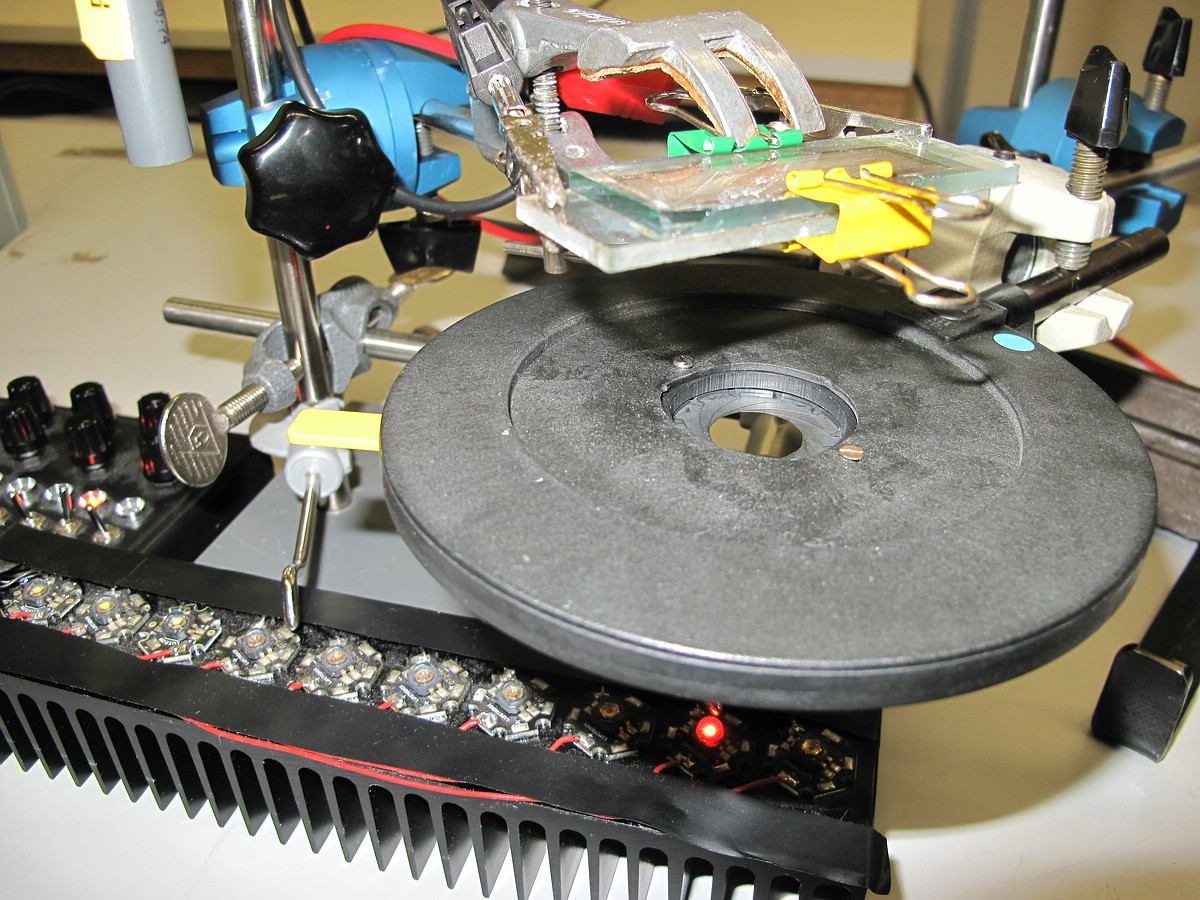
\includegraphics[width=0.7\textwidth]{./images/prIMG_3497.jpg}
\caption{Gr\"atzelzelle, beleuchtet von einer LED}
\end{center}
\end{figure}
}
\subsection[]{MHD-Generator}
\frame
{
\frametitle{MHD-Generator}
\begin{figure}
\begin{center}
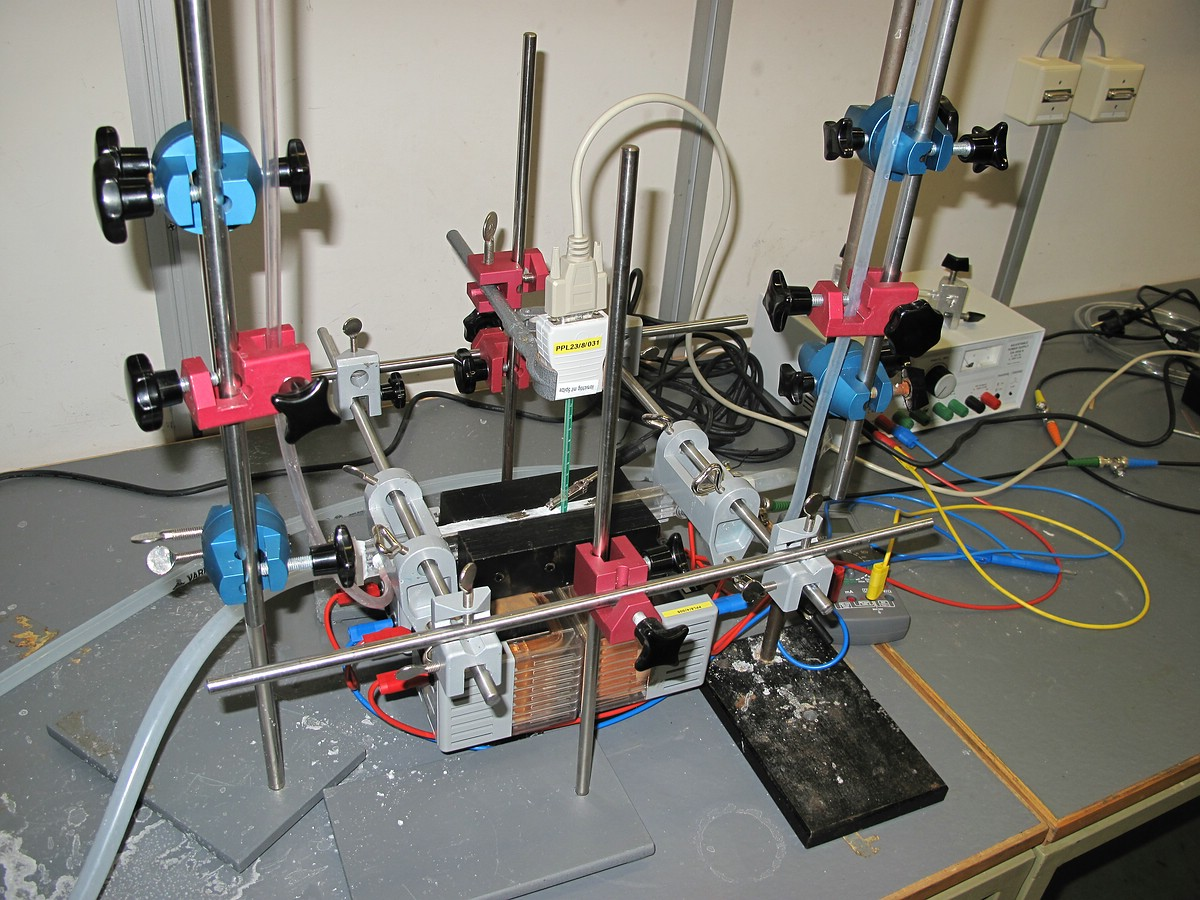
\includegraphics[width=0.7\textwidth]{./images/prIMG_3768.jpg}
\caption{MHD-Generator mit Zelle im Magnetfeld}
\end{center}
\end{figure}
}
\subsection[]{Direkte Messung der Erdrotation}
\frame
{
\frametitle{Direkte Messung der Erdrotation}
%\begin{SCfigure}
\begin{figure}
\begin{center}
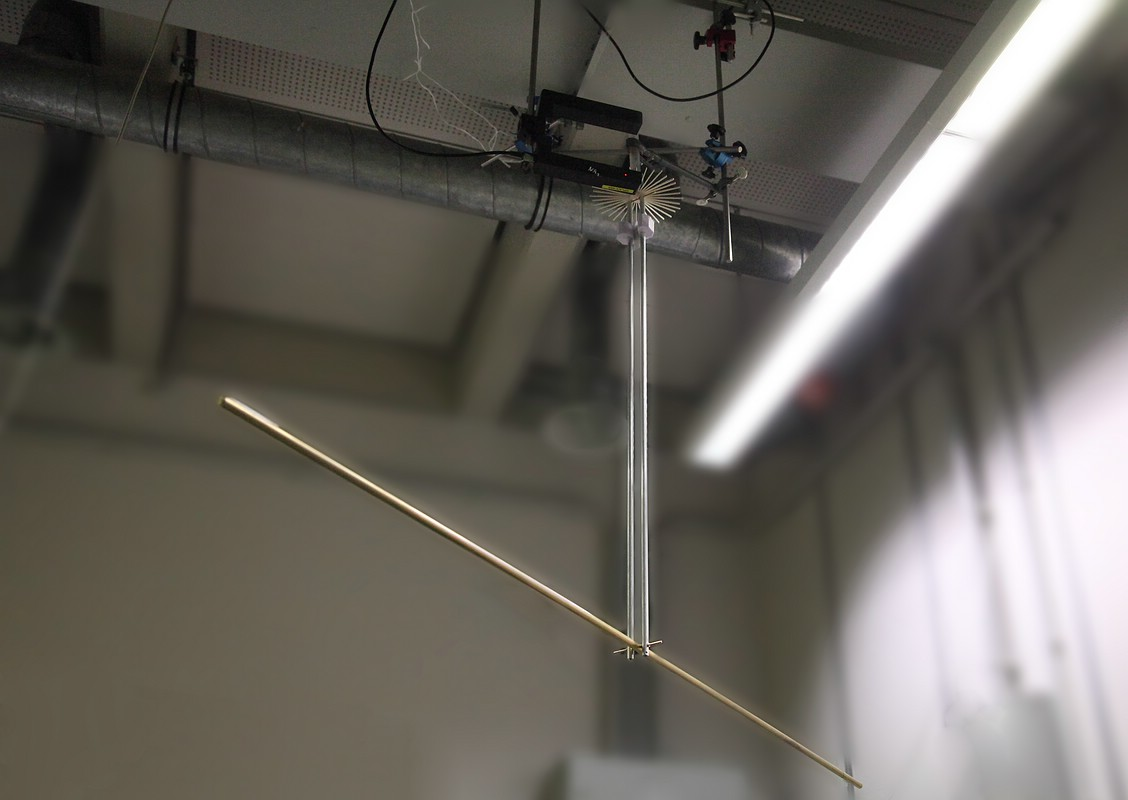
\includegraphics[width=0.8\textwidth]{./images/stab-gauss.jpg}
\caption{Rotierender Stab mit variablem Tr\"agheitsmoment}
%% des geht noch net wirklich, entweder des endgueltige bild is quer oder ich ueberleg mir dann was wenns so weit is...
%%% Querbild, etz gehts-Axi
\end{center}
\end{figure}
%\end{SCfigure}
}

\end{document}
